\documentclass[a4paper,oneside,12pt,english,brazil]{article}
\usepackage{lmodern}                            % Usa a fonte Latin Modern
\usepackage[T1]{fontenc}                        % Selecao de codigos de fonte.
\usepackage[utf8]{inputenc}                     % Codificacao do documento (conversão automática dos acentos)
\usepackage[margin=1.5cm]{geometry}
\usepackage{epsfig}
\usepackage{amsmath}
\usepackage{amssymb}
\usepackage{color}
\usepackage[pdftex,
            pdfauthor={Diego Rabatone Oliveira},
            pdftitle={\#TrilhaSP - Press Release},
            pdfsubject={Projeto \#TrilhaSP},
            pdfkeywords={transporte;mobilidade;aplicativo;mobile;gps;social;software livre;free software},
            pdfproducer={Latex with hyperref},
            pdfcreator={pdflatex}]{hyperref}
\begin{document}
\pagenumbering{gobble}%
\begin{figure}[Htb]
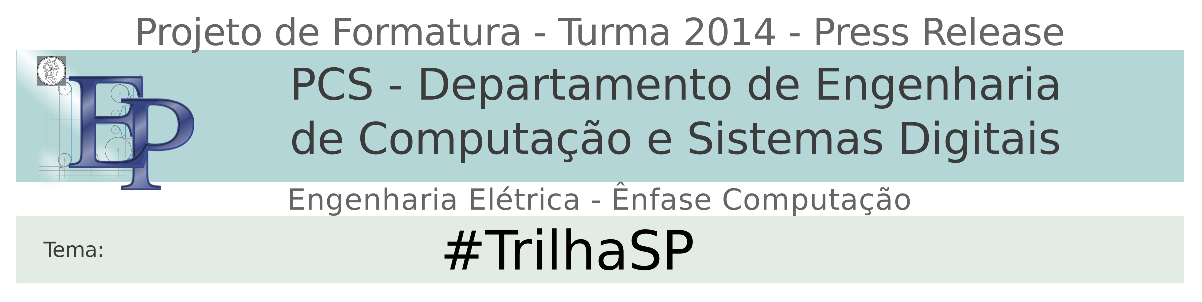
\includegraphics[width=\textwidth]{header.eps}
\end{figure}
A mobilidade urbana é hoje um dos mais latentes problemas das grandes cidades de todo o mundo. Em 2010, considerando 439 áreas urbanas nos Estados Unidos, os congestionamentos fizeram com que os motoristas gastassem 4,8 bilhões de horas e comprassem 7,2 bilhões de litros de combustível além do necessário, a um custo de 101 bilhões de dólares. Já em 2011, esses subiram para 5,5 bilhões de horas, 11 bilhões de litros de combustível e 121 bilhões dedólares. Assim, percebe-se que não só identificam-se altos custos sociais, ambientais e econômicos, como também estes custos são crescentes. A realidade brasileira não é muito diferente. De 2004 a 2007 o tempo de congestionamento de 4 das maiores cidades brasileiras (São Paulo, Rio de Janeiro, Belo Horizontee Porto Alegre) cresceu a uma taxa anual média de 16\%. Se considerarmos ainda as políticas públicas de incentivo ao mercado automobilístico, mais especificamente a redução do Imposto sobre Produtos Industrializados (IPI) para automóveis implementadas iniciada em maio de 2012, pode-se esperar que o crescimento do índice de congestionamento tenha sido até maior.

Atualmente existem diversos aplicativos que, majoritariamente, disponibilizam  aos usuários informações fornecidas pela API da  SPTrans. Isso se traduz em serviços de escolha de linha de ônibus, determinação de rotas e verificação de localização de ônibus com retorno também de tempo estimado para chegada.
Porém, não foi encontrado aplicativo que integrasse esse tipo de informação à avaliação por parte dos usuários sobre elementos-chaves do sistema, ou mesmo que utilize ``inteligência social'' obtida da massa de usuários para melhores decisões.

Assim surge o \#TrilhaSP, que é um aplicativo que se propõe a melhorar o fluxo de informações entre usuário e prestador de serviço público de transporte, tanto fornecendo aos gestores avaliações do sistema realizadas pelos usuários quanto disponibilizando aos usuários informações para uma tomada de decisão mais consciente ao utilizar o sistema de transporte.
Com o \#TrilhaSP os usuários do sistema público de transporte poderão avaliar o serviço, segundo critérios qualitativos como ``o ônibus estava muito lotado'', ``fui bem atendido pelo motorista'' e ``o ônibus estava sujo''. A opção por estes critérios qualitativos se deu pois identificou-se que eles influenciam na decisão do usuário sobre o modo de transporte preferido e não são facilmente mensurados por meio de tecnologias de automação, como é o caso da velocidade e frequência dos ônibus. Essas avaliações, que podem ser positivas ou negativas numa escala contínua, permitirão a criação de indicadores por ônibus que poderão ser utilizados pelas autoridades para melhorar o serviço e também influenciar no sistema de remuneração das empresas prestadoras de serviço. O módulo ``Mapa'' mostrará aos usuários um mapa com todos os usuários conectados, o que permitirá ao usuário optar por ir ou não para o ponto de ônibus num determinado horário usando a informação de demanda e ``lotação'' do ponto naquele momento, o que pode melhorar a distribuição da demanda no sistema, e levar a uma melhora do serviço prestado. Por fim, o módulo ``game'' tem por objetivo tanto atrair e reter os usuários no aplicativo quanto ser uma solução educativa, levando ao usuário informações e vivência verossímeis à realidade do sistema de transporte, como custo de um ônibus, necessidade de manutenção, etc.

O projeto foi desenvolvido utilizando tecnologias livres e também terá seu código fonte distribuído livremente.
Para mais informações visite: \url{http://trilhasp.datapublika.com}

\noindent
\hrulefill

\noindent
Autor: Diego Rabatone Oliveira <\href{mailto:diraol@diraol.eng.br}{diraol@diraol.eng.br}>

\noindent
Orientador: Prof. Dr. Reginaldo Arakaki <\href{mailto:reginaldo.arakaki@poli.usp.br}{reginaldo.arakaki@poli.usp.br}>

\noindent
Co-orientadora: Eng$^{a}$ Haydée Svab <\href{mailto:hsvab@hsvab.eng.br}{hsvab@hsvab.eng.br}>
\end{document}